% evaluation of the irradiance traces for the roof all of the district

% evaluation of the 75 percentile for the traces


% Find all the possible position inside the available surface, sort them by the 75-th percentile, eliminate the panel with percentile lower than a threshold, find the configuration for the panels them taking into account distance between panels and height difference (description of the algorithm)

% Given the best configurati23 lug 2021on try to place the same amount of panels on the used roof in a more classical way (classical algorithm description)

% evaluate the roi given the panel costs the maintenance cost and the production

% specificare meglio didascalia delle imaggini e rimpicciolirle
% \hline
The goal of the paper is to find the best possible configuration for a PV installation for a district of a city, considering the possibility to connect panel across contiguous roofs. The solution adopted to achieve this result is based on 5 main steps. %, summarized in Figure \ref{fig:methodology}. %This problem is novel w.r.t. state of the art works, like \cite{8342049}
The first step identifies the area of the district suitable for the installation of PV panels. Then we proceed with the generation of the traces of G and T for the whole area with a fine time and space resolution (A). In the second step we evaluate a statistical measure to find which points of the suitable area are the most illuminated during the year, and thus the most promising from the perspective of power production (B). The third step consist in the placement of PV modules to find the optimal configuration (C). Given such a placement,  we evaluate the yearly production (D) and the payback time (E) to allow comparison between different solutions.

\begin{comment}
\begin{figure}[th]
\centering
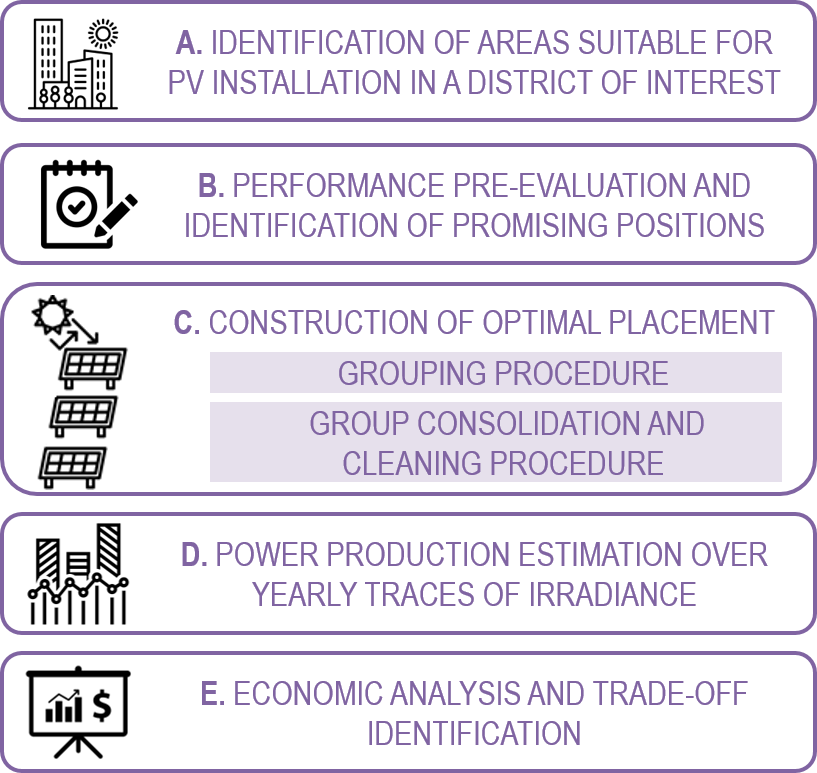
\includegraphics[width=\linewidth]{images/methodology.png}\vspace{-0.3cm}
\caption{Methodology adopted by the proposed framework to find the best possible configuration for a PV installation for a district of a city.}
%\vspace{-0.5 cm}
\label{fig:methodology}
\end{figure}
\end{comment}


\subsection{Suitable area and irradiance}
\label{subsec:suitablearea}
Starting from a Digital Surface Model (DSM) of the district, the algorithm identifies possible encumbrances and the corresponding evolution of  shadows to find areas which could be used for the panel deployment. 

To extract such areas, we used GDAL\cite{gdal} to process the DSM and identify the surfaces (i.e., roofs) that maximize power production in terms of tilt angle and orientation depending on the geographic location of the district. In our case study, we generated two \attenzione{.tiff files} one to store the data of the slope and the other to store the data of the aspect for the area under test. Thenwere processed this two files  to extract the surfaces with a slope between 15 and 36 degrees and aspect value between 240 and 300 degrees in order to have roof pitches oriented towards South, configuration that guarantees optimal sun exposition and potential PV production \cite{tilt}. Figure \ref{fig:buildvssuit} shows how the area that is suitable for PV installation resulting from this step is only a portion with respect the whole district area.
% This step also allows us to know the inclination and the aspect of the roof that will be used in the following steps of the procedure to consider the inclination of the pv panels.

Each identified suitable area is then annotated with the inclination and the aspect of its roof pitch. Those area are then intersected with the cadastral data to annotate the medium height of the roofs, this is an important detail because the height differences of the roof needs to be taken into account when the placement algorithm is executed. The area are then sampled with the same same resolution of the DSM (i.e. 1m), the result of this sampling is shown in Figure \ref{fig:buildvssuit}. Using these points we are able to determine the evolution of irradiance over time from yearly weather data and the shadow model developed in \cite{7997730}. The usage of georeferenced points allows us to generate and store the data data only for the areas that could actually be exploited for the installation of the pv panels while achieving a fine-grain representation of the solar evolution of the suitable areas over time., 
%After the traces calculation we evaluate the 75-th percentile for each point of this suitable area, these values allows us to identify the more illuminated points to be used for the PV panel placement. The Figure \ref{fig:buildvsperc} show the result of this second step, whiter points corresponds to higher value of the 75-th percentile.

\attenzione{Non annotiamo anche l'altezza del tetto per i vincoli dell'algoritmo?}

\attenzione{Non stiamo più usando la griglia, come faccio allora a costruire le tracce? Con che granularità o come lavoro?}

\subsection{Performance pre-evaluation}
The next step consists of identifying the most irradiated portions of the suitable areas, that are the most promising positions for the installation of PV modules. To get a compact signature for each \attenzione{DSM point}, we use the \emph{75th percentile of irradiance}, i.e., the
value below which 75\% of the yearly irradiance traces fall: larger values of the percentile identify positions whose irradiance trace distribution is more skewed towards the upper range of the irradiance values, i.e., that are more irradiated and more promising for PV power production. 
%For each point in the suitable area \attenzione{vedi sopra, quale punto?}, we evaluate the 75-th percentile of its irradiance trace, value that according to the analysis in \cite{8342049} allows  
The 75th percentile thus allows to discriminate between highly irradiated and poorly irradiated portions \cite{8342049_OMITTED}. Figure \ref{fig:buildvsperc} shows the result of this second step: the suitable area identified in Figure \ref{fig:buildvssuit} is now colored so that whiter points corresponds to a higher value of the 75th percentile (i.e., more irradiated points). 

The \attenzione{DSM points} are then sorted by decreasing value of the 75th percentile. The user is now allowed to give a threshold value $minTh$ representing the minimum value of the percentile that is accepted for PV placement. The experimental analysis will prove the impact of this choice on the resulting identified solution. All positions with 75th percentile lower than $minTh$ are now excluded from the suitable area, as the performance indicator identifies them as non-promising locations from the perspective of PV power generation. The resulting suitable area now represents the area that can be occupied by PV modules to achieve optimal power generation.  
% This part finds possible places where a single panel could be placed, the dimension of the panel to consider and the resolution of the search, that can be defined by the user, are taken into account to produce a list of exploitable positions. For each of these possible position we calculate a performance indicator as the minimum 75-th percentile of the points, represented in Figure \ref{fig:buildvsperc},that intersect the panel surface. Then we sort the list of those positions according to that value.
%For this list of panels positions we define than a threshold value $minTh$ for the performance indicator to limit the number of positions to consider for the following steps.

\subsection{Optimal Placement algorithm \attenzione{DA SISTEMARE, NE DOBBIAMO PARLARE LUNEDì}}
\label{subsec:greedyplacement}
The third part of the algorithm uses the list of panels positions found in the previous step to identify an optimal panel configuration. This part is divided in two different procedures that are iterated until the list of possible panel positions it is empty.

\attenzione{Questa procedura viene ripetuta un tetto alla volta giusto? Questa parte non è chiara e invece è il cuore del paper!!!}

\subsubsection{Grouping procedure}The algorithm selects the first available position (with highest available irradiance according to the sorting) 


Starting from the first position of the list the algorithm proceeds iteratively along the list to find the next panel to select by checking three conditions:
\begin{itemize}
    \item The next panel should not intersect with any of the panels selected previously.
    \item It is not on one of the roofs used by the previous iterations
    \item It should not be farther than a maximum distance \emph{maxD} from the previous panel.
    \item The difference in height from the previous panel should not be greater than a distance \emph{maxH}
\end{itemize}
If a panel does not respect the first or the second condition it is completely removed from the list and will not be used for the next iterations. If instead a panel does not respect the third or the fourth condition it is temporarily removed and if it survives to the list cleaning procedure it will be considered again for the following iterations.
The numbers \emph{maxD} and \emph{maxH} can be defined by the user according to his preference or the needs of the scenario. The algorithm will proceed until it is not able to place any other panel on the same area thus the group is considered completed and it is used as input for the next procedure.
\subsubsection{Group consolidation and list cleaning procedure}
To consolidate the group the algorithm considers only an amount of panel multiple of \emph{S}, that is the number of panel in a series that the user has defined, all the panels in excess are discarded forever.
The ID number of the roof used for the panel of that group is stored and to avoid to use the same roofs in the next iterations (see condition 2 in the grouping procedure).
Then all the panels that were discarded due to the third or the fourth conditions of the grouping procedure and inserted again in the list of panels that will be used again for the grouping procedure.

\subsection{Power production}
The last step is the evaluation the yearly power production for the identified optimal PV installation. To achieve a measure of performance, the algorithm generates also a traditional placement of the same number of PV modules, by positioning them in the suitable area but with a more standard positioning (i.e., a \virgolette{compact} rectangular placement that does not consider the 75th percentile of irradiance). %Consider that the traditional placement is positioned in the suitable area and thus benefits from the analysis of irradiance and of shadow distribution, thus being a competitive placement.  

Given a placement (either the generated optimal one or the traditional one), we determine the yearly power production of each PV module. For each module, the yearly irradiance trace is determined by \attenzione{considering the traces for the DSM point covered by the PV module}. In case there are multiple points, for each time instant we consider the minimum value of the irradiance over all the traces, to reproduce the bottleneck effect described in Section \ref{sec:back_pv}. % to build the traces.
% both the configuration (i.e. optimal, classical). In order to do so we find the irradiance trace for each single panel by intersecting the result of the step C and D with the result of the step A. In case there are multiple points that belong to the same panel, for each time instant we will consider the minimum value of the irradiance to build the traces.

Once the yearly trace for each PV module has been evaluated, we estimate the yearly power production of the overall PV installation by considering the series and parallel connections between PV modules. Given $n$ the number of groups identified in step \ref{subsec:greedyplacement} and $m$ the number of PV modules composing each group, the resulting power $P_{yearly} = V_{yearly} \cdot I_{yearly}$ of the whole installation is thus derived with the following formula, reproducing the bottleneck effect mentioned in Section \ref{sec:back_pv}:
\[  \left\{
		\begin{array}{rcl}
V_{panel} & = & \min_{j=1,\dots,n} (\sum_{i=1,\dots,m} V_{module,ij})\\
I_{panel} & = & \sum_{j=1,\dots,n} (\min_{i=1,\dots,m} I_{module,ij})\\
\end{array}
\right.
\]
where $V_{module,ij}$ and $I_{module,ij}$ are the
voltage and current extracted from the $i$-th PV module in the $j$-th string, and $T$ is the length of the irradiance traces. 
%$$P_{yearly} =\sum_{i = 1..N}P^i_{yearly}=\sum_{i = 1..N} \sum_{t = 1 ... T} V^i_{array}(t) \cdot I^i_{array}(t)$$
%where $T$ is the length of the irradiance traces and $N$ the number of the groups obtained in the step \ref{subsec:greedyplacement}. 

\subsection{Economic analysis}
\label{sec:economic}
The economic effectiveness of a PV installation is usually determined as its financial Payback-Time (PT), i.e., how much time it takes for the total savings and revenue streams to cover the total cost of the initial installation. %In this work we used as the Payback-Time (PT) as a performance metric for the different configuration. 
It thus indicates the number of years of operation needed to payback the initial investment when considering also maintenance costs by using the following formula:

$$PT=\frac{I_c}{{R_y}-{M_y}}$$
Where $I_c$ is the installation cost, $R_y$ are the yearly revenue generate by selling all the energy produced to the grid (calculated by multiplying the yearly kWh production $P_{yearly}$ of a configuration per $E_p$ that is the price at which the energy is sold to the grid), $M_y$ is the yearly maintenance cost due to the price of cleaning, monitoring, and repairing that needs to be applied periodically an efficient system.



% RInforzare descrizione dati DSM etc, spiegare come si gestiscono i dati 

% All'inizio dell'introduzione mettiamo in evidenza il fatto che consideriamo tetti contigui di edifici diversi. Sottolineare come sia cambiato il metodo di gestione dei dati per ovviare alle limitazioni dovute dall'upscaling citare tsusc 
